\section{Valutazione}\label{sec:valutazione}

Questa sezione verifica i requisiti e misura quanto costano, in gas, tempo e spazio, le scelte di sicurezza. Le misure sono raccolte da script che usano il codice reale del progetto e analizzate in un notebook Jupyter (cartella \texttt{analisi/}), che rigenera tutte le figure.

\subsection{Verifica dei requisiti}
\begin{table}[H]
\centering\footnotesize
\renewcommand{\arraystretch}{1.2}
\begin{tabular}{@{}p{.07\textwidth}p{.13\textwidth}p{.72\textwidth}@{}}
\toprule
Req. & Stato & Evidenza\\
\midrule
RF1 & Soddisfatto & Registrazione e login con passkey, anche ML-DSA-44 (sez.~\ref{sec:fido2}).\\
RF2 & Soddisfatto & Consenso per finalità con scadenza e revoca nel contratto, concesso e revocato dal paziente con il proprio wallet (sez.~\ref{sec:consenso-paziente}).\\
RF3 & Soddisfatto & Ruolo di medico assegnato dalla struttura e consenso per la finalità verificati a ogni accesso (sez.~\ref{sec:accesso}).\\
RF4 & Soddisfatto & Ogni accesso, concesso o negato, e ogni referto firmato sono registrati sulla catena; i tentativi d'emergenza respinti nel registro cifrato.\\
RF5 & Estensione & Progettata ma non realizzata nel prototipo (sez.~\ref{sec:zkp}).\\
RF6 & Soddisfatto & Referti cifrati con schema ibrido post-quantistico; sulla catena solo pseudonimi e impronte (sez.~\ref{sec:dati}).\\
RF7 & Soddisfatto & Il paziente consulta il proprio registro e lo verifica sulla catena con il proprio wallet (sez.~\ref{sec:registro-paziente}); l'auditor con \texttt{npm run registro-accessi}.\\
RF8 & Soddisfatto & Accesso d'emergenza con ruolo dedicato e motivazione obbligatoria.\\
RF9 & Soddisfatto & Revoca delle passkey e uscita da tutti i dispositivi (sez.~\ref{sec:fido2-revoca}).\\
RF10 & Soddisfatto & Referti firmati con la passkey e verificati a ogni consegna (sez.~\ref{sec:firma}).\\
\midrule
RNF1 & Soddisfatto & Phishing e replay respinti in tutte le prove (sez.~\ref{sec:val-attacchi}).\\
RNF2 & Soddisfatto & AES-256-GCM con chiave protetta da ML-KEM-768 e X25519.\\
RNF3 & Soddisfatto & Registro on-chain in sola aggiunta; dettagli off-chain legati all'impronta.\\
RNF4 & Soddisfatto & Finalità e minimizzazione applicate; cancellazione su richiesta con conservazione dei soli dati dovuti (sez.~\ref{sec:cancellazione}).\\
RNF5 & Soddisfatto & Pattern di sicurezza e 36 test sui contratti (sez.~\ref{sec:test}).\\
RNF6 & Soddisfatto & Costo costante e contenuto per ogni operazione (sez.~\ref{sec:val-gas}).\\
RNF7 & Soddisfatto & Senza audit nessuna consegna e nessun salvataggio (sez.~\ref{sec:accesso}).\\
\bottomrule
\end{tabular}
\caption{Stato dei requisiti.}
\end{table}

\subsection{Metodo e ambiente di misura}
Tre script producono i dati in formato CSV: \texttt{blockchain/scripts/gas.ts} misura il gas dei contratti sulla rete di Hardhat, \texttt{backend/bench/crypto.ts} firme, cifratura e Argon2id con le funzioni del server, \texttt{backend/bench/attacks.ts} ripete gli attacchi del modello di minaccia contro il backend reale con archivi in memoria. Le parti casuali usano un seme fisso, quindi l'analisi è ripetibile.

Tutte le misure sono state generate con lo script \texttt{analisi/genera.sh} sul portatile di sviluppo, con processore Intel Core Ultra~7~355 (8 core) e 7~GiB di memoria assegnati a WSL2, Node.js~24 e OpenSSL~3.5. Il gas e gli esiti degli attacchi non dipendono dalla macchina; i tempi sì, e vanno letti come ordini di grandezza e confronti relativi.

\subsection{Costi on-chain}\label{sec:val-gas}
La figura~\ref{fig:gas} riporta il gas di ogni operazione, misurato su 150 pazienti diversi. La registrazione di un accesso costa circa 42 mila unità di gas se concesso e 35 mila se negato; un consenso nuovo circa 50 mila, il suo rinnovo 33 mila, la revoca 25 mila. Le differenze dipendono dal costo della memoria in Ethereum: scrivere uno slot vuoto costa più che aggiornarne uno già usato, per questo anche la prima voce del registro costa di più (59 mila). Il grafico di destra mostra il risultato più importante per la sicurezza: il costo non cresce con il numero di pazienti o di voci, perché nessuna operazione contiene cicli su dati non limitati, quindi un attaccante non può causare un DoS per esaurimento del gas riempiendo i registri. La pubblicazione dei due contratti costa in tutto circa 3,7 milioni di unità di gas.

\begin{figure}[H]
\centering
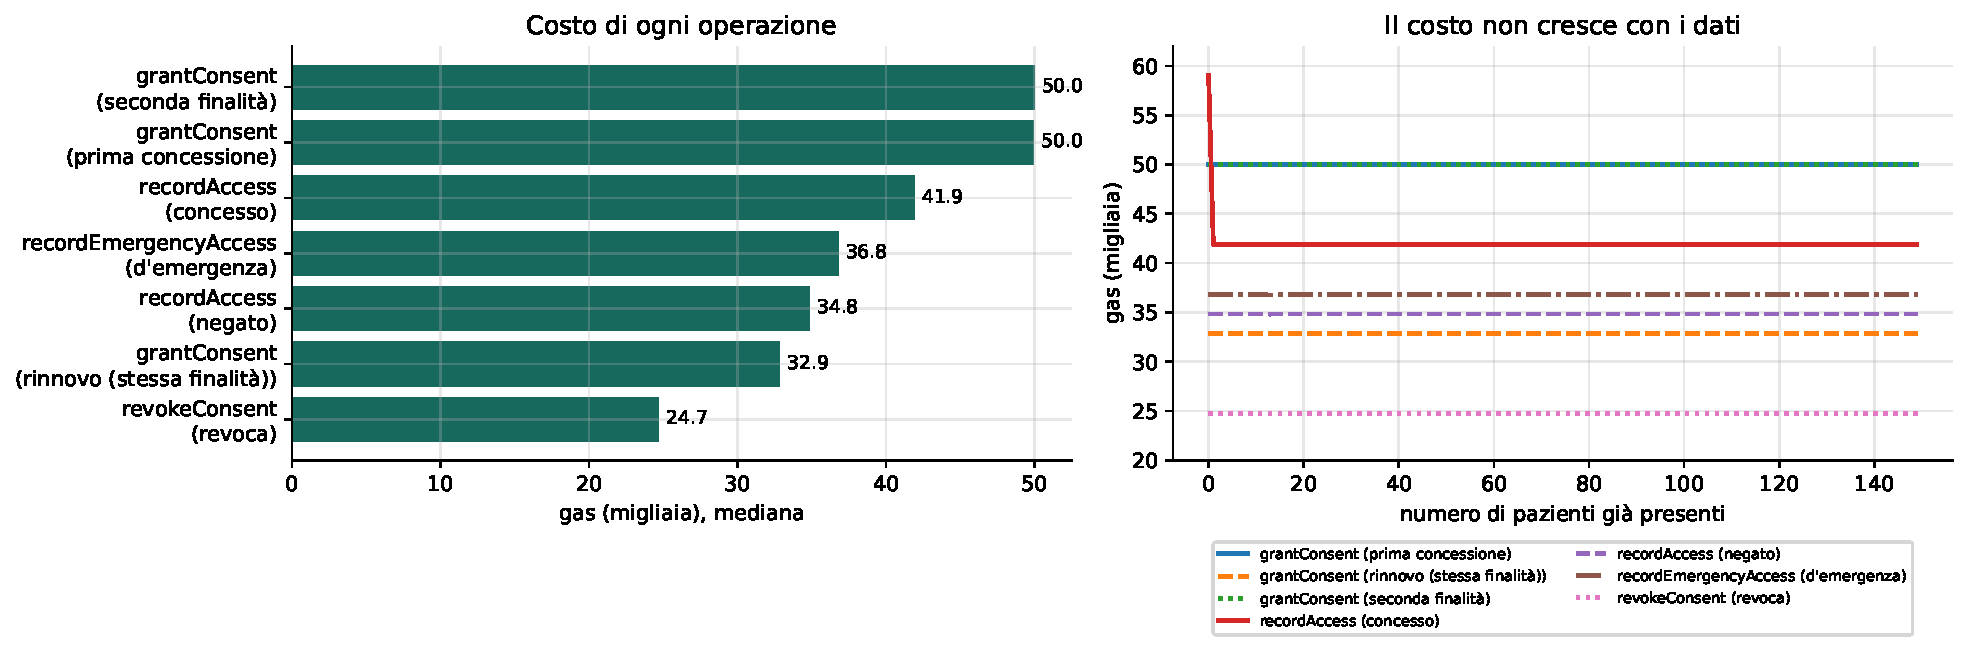
\includegraphics[width=\textwidth]{figure/gas_operazioni.pdf}
\caption{Gas di ogni operazione (a sinistra) e andamento al crescere dei pazienti (a destra).}\label{fig:gas}
\end{figure}

Il costo in euro dipende dal prezzo del gas e dell'ether, che variano di continuo, e dal volume di utilizzo. La figura~\ref{fig:gas-anno} lo calcola in forma parametrica, con ipotesi dichiarate (1 ETH = 3000~€, 50 consensi e 10 revoche al giorno). Con mille accessi al giorno il costo annuo va da qualche migliaio di euro con il gas a 0,1~gwei a quasi un milione con il gas a 20~gwei. È un argomento in più, accanto alla riservatezza dei metadati, a favore di una rete \emph{permissioned} o di secondo livello.

\begin{figure}[H]
\centering
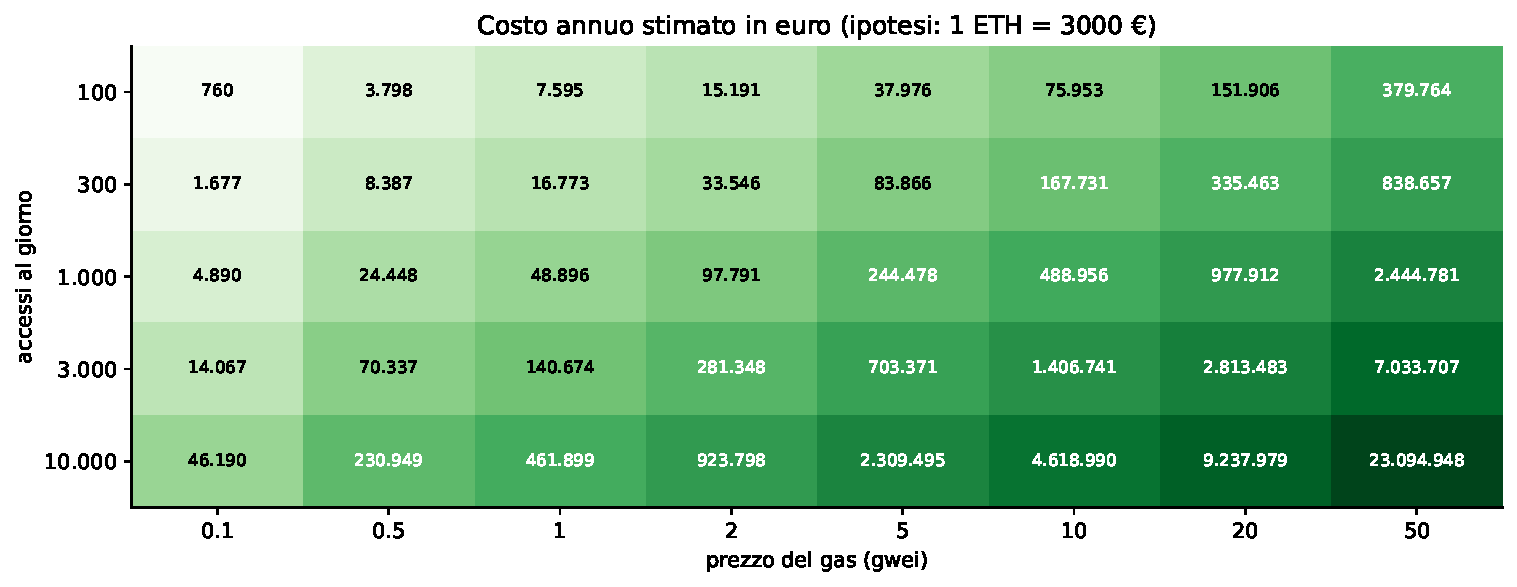
\includegraphics[width=.92\textwidth]{figure/gas_costo_annuo.pdf}
\caption{Costo annuo stimato al variare del prezzo del gas e degli accessi giornalieri (ipotesi dichiarate nel notebook).}\label{fig:gas-anno}
\end{figure}

\subsection{Firme classiche e post-quantistiche}
La figura~\ref{fig:firme} confronta le passkey ES256 e ML-DSA-44 su 300 firme ciascuna. Il prezzo della sicurezza post-quantistica sta quasi tutto nello \textbf{spazio}: la chiave pubblica passa da 77 a 1322 byte, la firma da 71 a 2420, la risposta WebAuthn completa da circa 500 a circa 3600 byte. Il tempo di verifica sul server resta invece dello stesso ordine, circa mezzo millisecondo per entrambi: per un login o per la firma di un referto non è un collo di bottiglia. La dimensione conta di più per i dispositivi con poca memoria e i protocolli con limiti sui messaggi.

\begin{figure}[H]
\centering
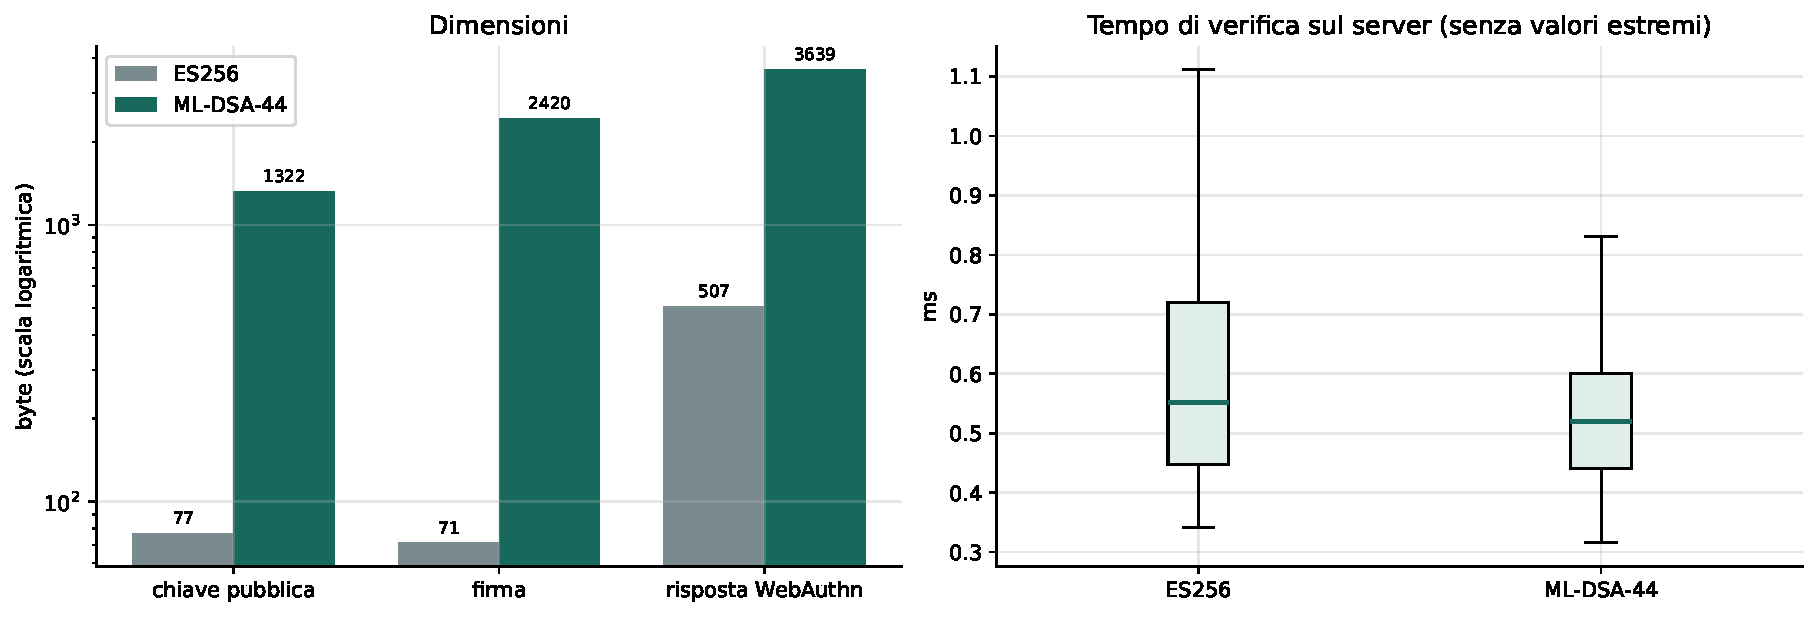
\includegraphics[width=\textwidth]{figure/firme_confronto.pdf}
\caption{Dimensioni (scala logaritmica) e tempo di verifica di ES256 e ML-DSA-44.}\label{fig:firme}
\end{figure}

\subsection{Cifratura ibrida}
Cifrare o decifrare un referto richiede circa 0,15~ms fino a 64~KiB e meno di un millisecondo per un referto di 1~MiB (0,84~ms per la cifratura, 0,56 per la decifratura; figura~\ref{fig:cifratura}). Per i referti piccoli il tempo è dominato dai due meccanismi di incapsulamento, che hanno costo fisso, per quelli grandi da AES-GCM. ML-KEM-768 e X25519 costano decine di microsecondi ciascuno (17 e 24 contro 53 e 33 per incapsulamento e decapsulamento): la componente post-quantistica non pesa sui tempi.

\begin{figure}[H]
\centering
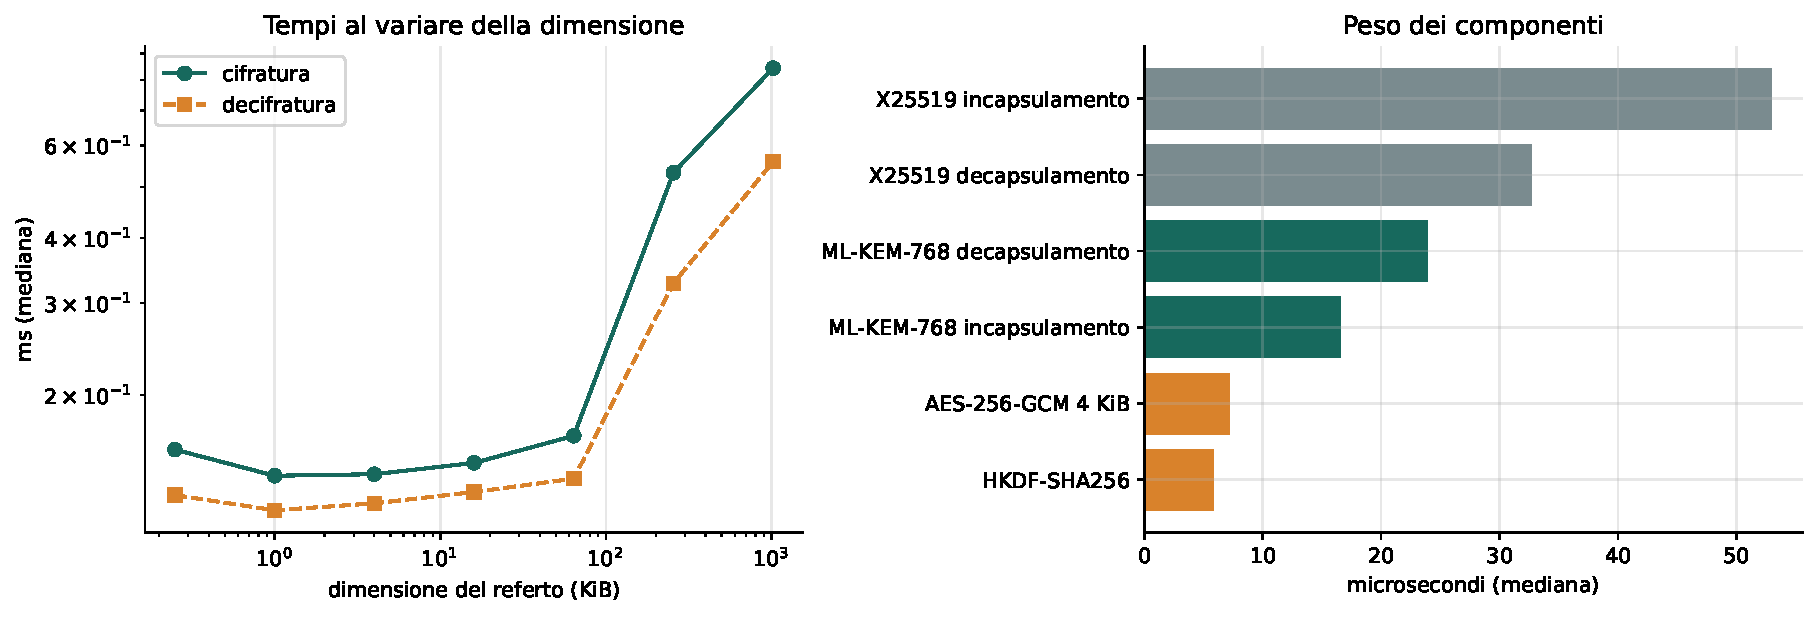
\includegraphics[width=\textwidth]{figure/cifratura_tempi.pdf}
\caption{Tempi di cifratura e decifratura al variare della dimensione del referto e peso dei singoli componenti.}\label{fig:cifratura}
\end{figure}

Per lo spazio (figura~\ref{fig:spazio}) lo schema aggiunge poco meno di 2~KB fissi, soprattutto per il testo cifrato di ML-KEM (1088 byte); i campi sono però salvati come testo base64, che aumenta ogni contenuto di un terzo anche per i referti grandi. Salvarli come dati binari di MongoDB eliminerebbe questo costo.

\begin{figure}[H]
\centering
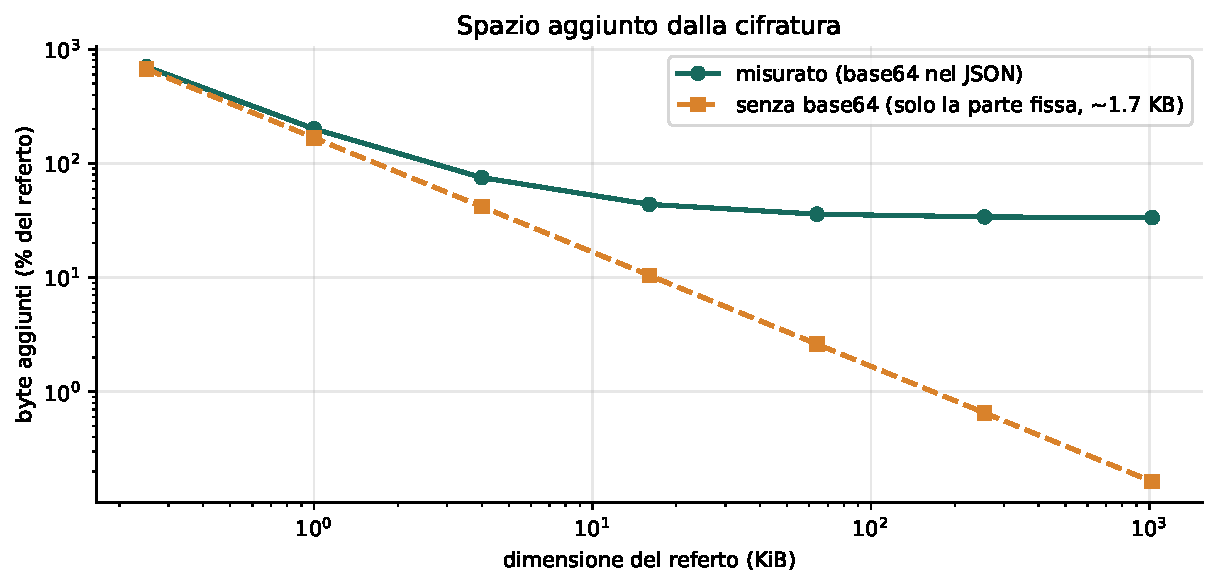
\includegraphics[width=.75\textwidth]{figure/cifratura_spazio.pdf}
\caption{Byte aggiunti dalla cifratura, in percentuale della dimensione del referto: misurati e senza la codifica base64.}\label{fig:spazio}
\end{figure}

\subsection{Custodia delle chiavi}
\paragraph{Argon2id.} Con i parametri del progetto (64~MiB, 3 passate) un tentativo di indovinare la passphrase costa circa 70~ms sulla macchina delle misure (figura~\ref{fig:argon}, a sinistra). A destra il tempo medio di una ricerca esaustiva, al variare della velocità dell'attaccante rispetto a quella macchina: con una passphrase di cinque parole scelte a caso da un dizionario di 7776 (circa 65 bit) servirebbero decine di migliaia di anni anche a un attaccante un milione di volte più veloce, mentre quattro parole (circa 52 bit) scenderebbero a pochi anni. La stima presuppone una passphrase scelta davvero a caso: il controllo sui 12 caratteri minimi non lo garantisce, e una frase nota o prevedibile ha un'entropia molto più bassa.

\begin{figure}[H]
\centering
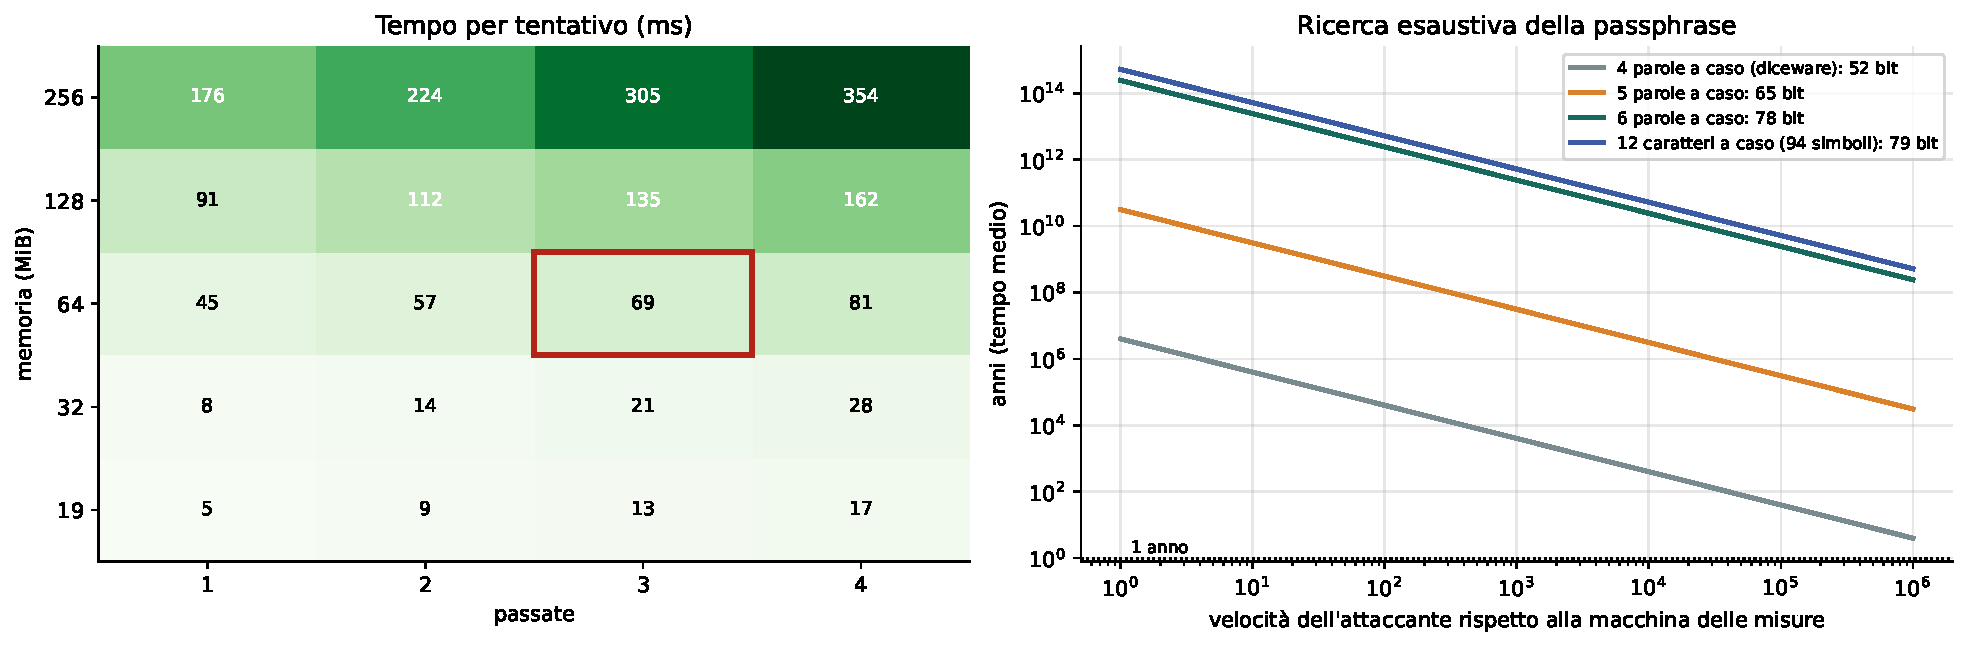
\includegraphics[width=\textwidth]{figure/argon2_costo.pdf}
\caption{Costo di un tentativo al variare dei parametri di Argon2id (in rosso la configurazione del progetto) e tempo medio di una ricerca esaustiva.}\label{fig:argon}
\end{figure}

\paragraph{Schema a soglia.} Per lo schema di Shamir si sono calcolate, con la distribuzione binomiale e una verifica Monte Carlo, la probabilità di perdere le chiavi (meno di $k$ custodi disponibili) e quella che vengano rivelate (almeno $k$ custodi compromessi), assumendo custodi indipendenti. La figura~\ref{fig:shamir} mostra che una copia unica è il caso peggiore su entrambi i fronti, che copie multiple senza soglia riducono la perdita ma moltiplicano il rischio di furto, e che una soglia piena fa il contrario. A destra, con l'ipotesi che ogni custode non sia disponibile nel 10\% dei casi e sia compromesso nel 5\%, il rischio peggiore tra i due è minimo per soglie intorno alla metà del numero di custodi; lo schema adottato, 3 su 5, porta entrambi i rischi sotto l'1\%.

\begin{figure}[H]
\centering
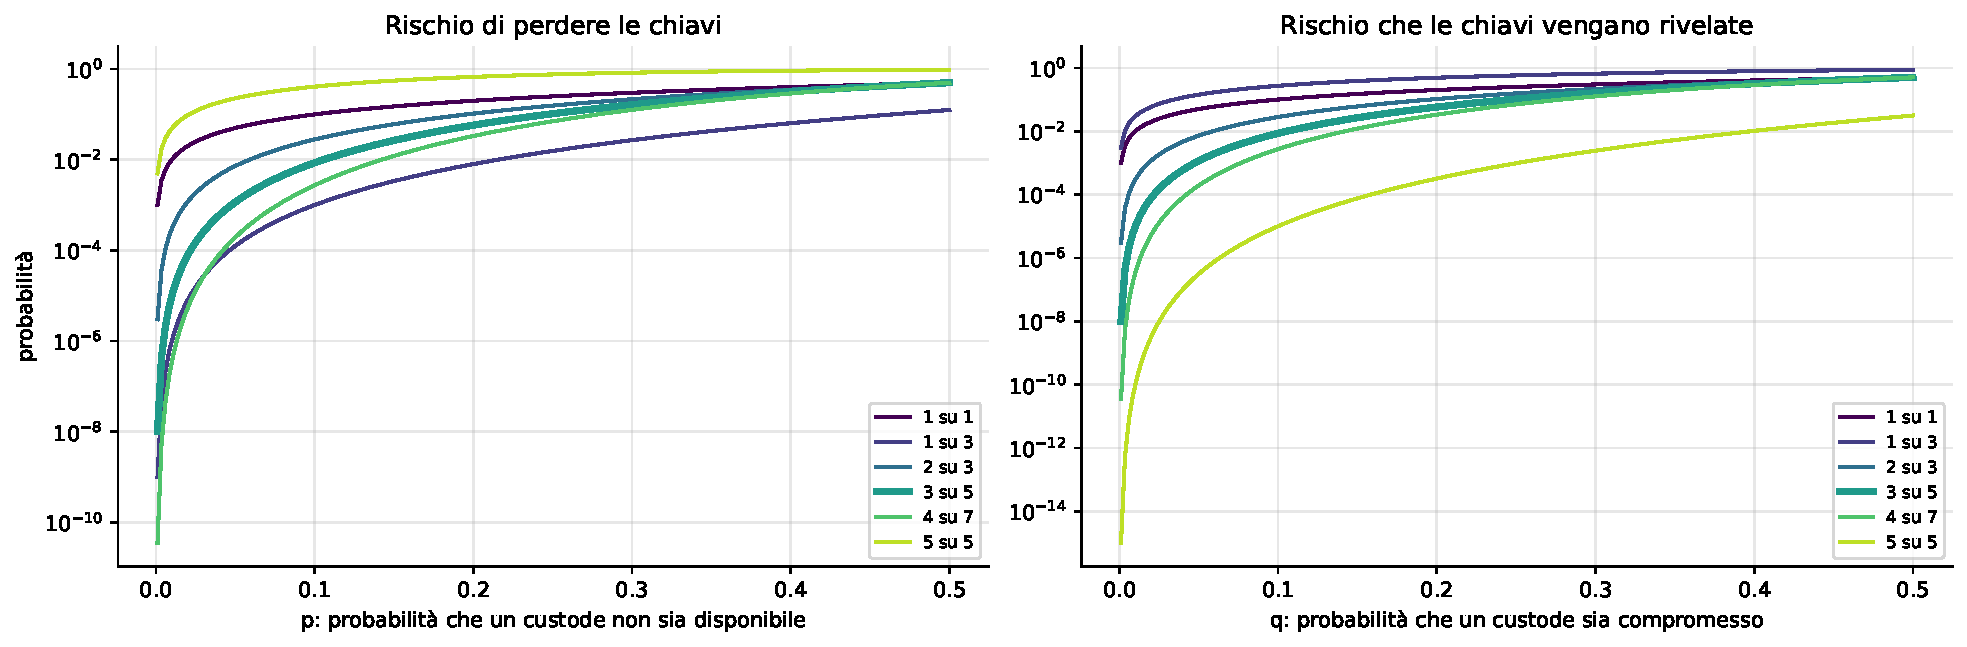
\includegraphics[width=\textwidth]{figure/shamir_rischi.pdf}\\[4pt]
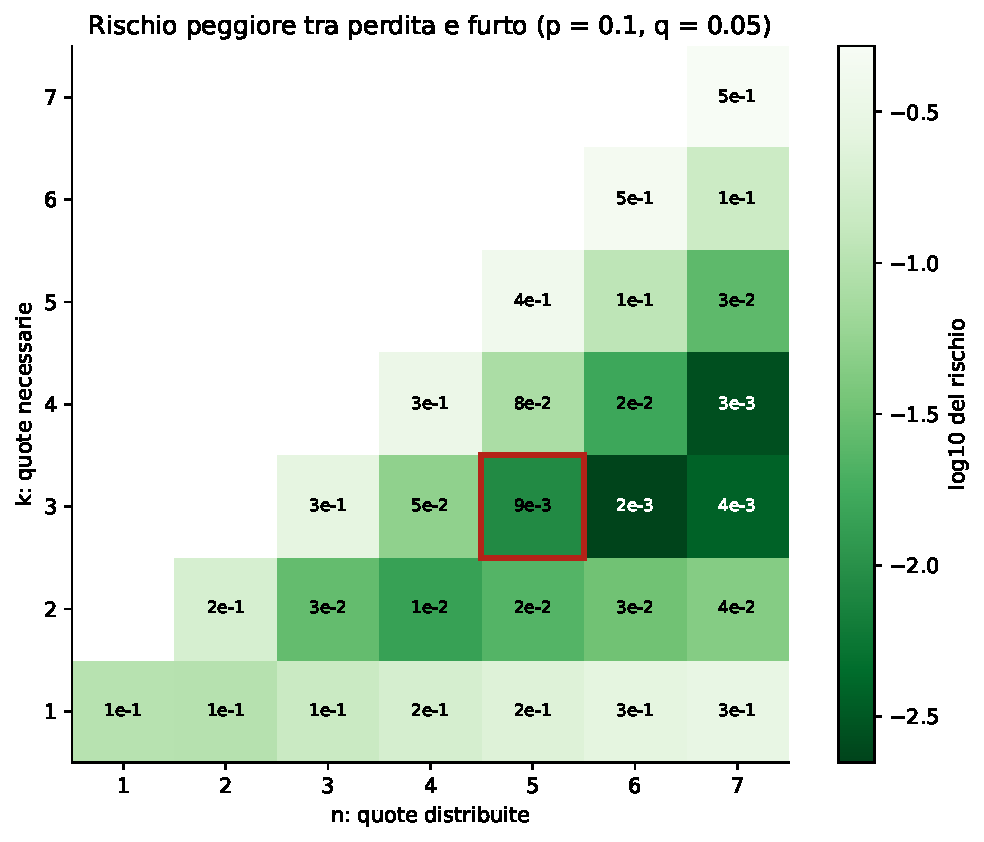
\includegraphics[width=.6\textwidth]{figure/shamir_griglia.pdf}
\caption{Rischio di perdita e di rivelazione delle chiavi per diversi schemi a soglia, e rischio peggiore tra i due per ogni scelta di $k$ e $n$ (in rosso lo schema del progetto).}\label{fig:shamir}
\end{figure}

\subsection{Campagne d'attacco}\label{sec:val-attacchi}
Ogni attacco del modello di minaccia è stato ripetuto 30 volte contro il backend reale, registrando sia l'esito dell'attacco sia quello dell'operazione legittima corrispondente: una difesa che blocca anche gli utenti onesti non è una buona difesa. Per controllare che le prove rilevino davvero i problemi, gli scenari di autenticazione sono stati eseguiti anche sul codice privo delle correzioni della revisione di sicurezza (figura~\ref{fig:attacchi}).

\begin{figure}[H]
\centering
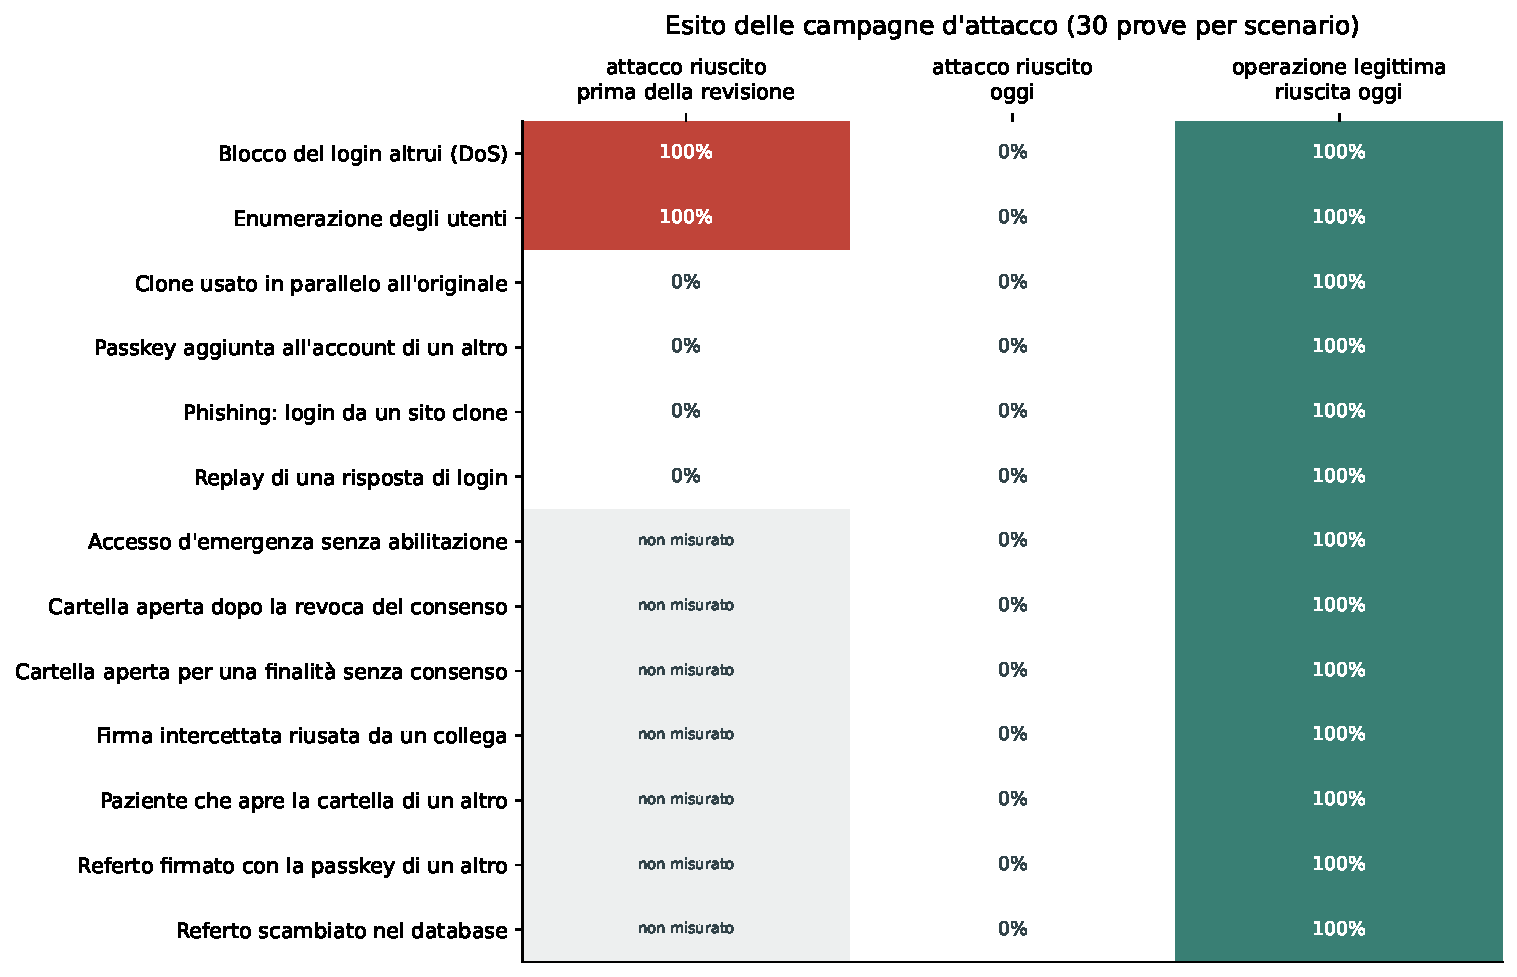
\includegraphics[width=.9\textwidth]{figure/attacchi_matrice.pdf}
\caption{Esito delle campagne d'attacco: percentuale di prove in cui l'attacco o l'operazione legittima sono riusciti.}\label{fig:attacchi}
\end{figure}

Nel prototipo nessun attacco riesce in nessuna prova e tutte le operazioni legittime riescono; senza le correzioni, il blocco del login altrui e l'enumerazione degli utenti riescono nel 100\% delle prove. La figura~\ref{fig:dos} mostra il blocco del login al crescere delle richieste dell'attaccante: senza correzione basta una richiesta al momento giusto, con la correzione la vittima entra sempre.

\begin{figure}[H]
\centering
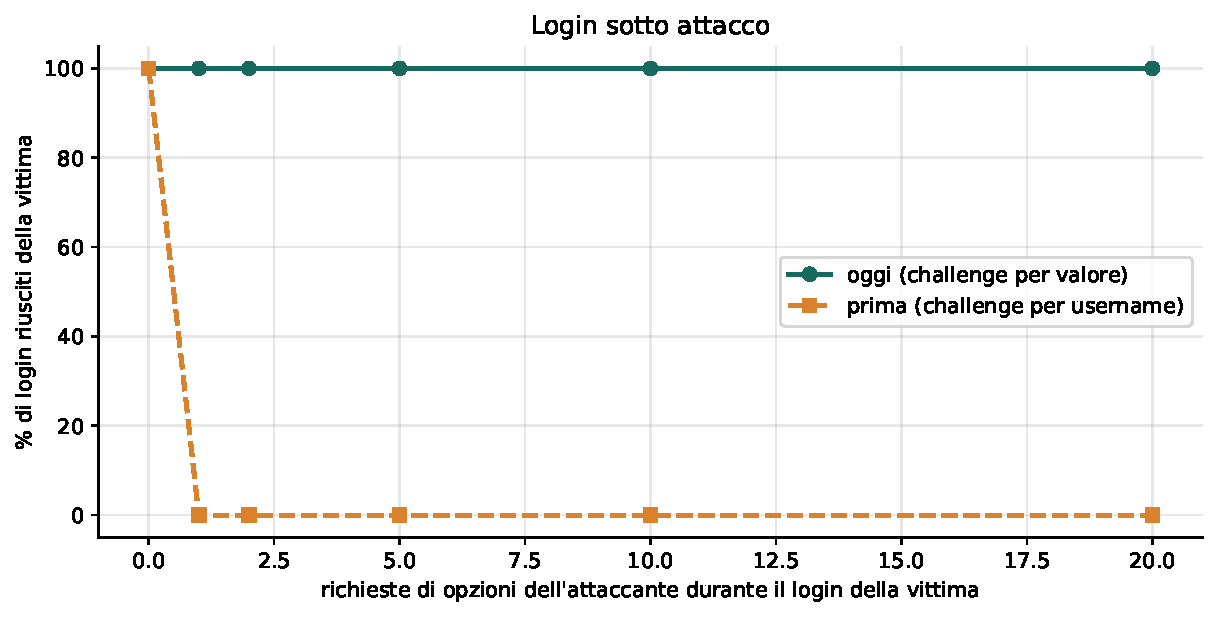
\includegraphics[width=.65\textwidth]{figure/login_dos.pdf}
\caption{Percentuale di login riusciti della vittima al crescere delle richieste dell'attaccante, senza e con la correzione.}\label{fig:dos}
\end{figure}

Zero successi su 30 prove non dimostrano che un attacco sia impossibile, ma che il controllo che lo blocca è sempre attivo, come atteso per controlli deterministici. Le campagne non sostituiscono un penetration test, ma rendono ripetibili le affermazioni di sicurezza della relazione.

\subsection{Limiti della valutazione}
\begin{itemize}
  \item I tempi sono misurati su un solo portatile; quelli della blockchain locale non rappresentano una rete reale, dove la conferma di un blocco richiede secondi, e non sono stati misurati.
  \item Il costo in euro e la stima di forza bruta dipendono da ipotesi esplicite: cambiandole cambiano i numeri, non il metodo.
  \item Il modello di Shamir assume custodi indipendenti; custodi che condividono un luogo o un sistema hanno guasti correlati e un rischio maggiore.
  \item Le campagne d'attacco usano archivi in memoria e una blockchain simulata; le proprietà che dipendono dal database sono coperte dai test d'integrazione su MongoDB.
\end{itemize}
